%%%%%%%%%%%%%%%%%%%%%%%%%%%%%%%%%%%%%%%%%
% Focus Beamer Presentation
% LaTeX Template
% Version 1.0 (8/8/18)
%
% This template has been downloaded from:
% http://www.LaTeXTemplates.com
%
% Original author:
% Pasquale Africa (https://github.com/elauksap/focus-beamertheme) with modifications by 
% Vel (vel@LaTeXTemplates.com)
%
% Template license:
% GNU GPL v3.0 License
%
% Important note:
% The bibliography/references need to be compiled with bibtex.
%
%%%%%%%%%%%%%%%%%%%%%%%%%%%%%%%%%%%%%%%%%

%----------------------------------------------------------------------------------------
%	PACKAGES AND OTHER DOCUMENT CONFIGURATIONS
%----------------------------------------------------------------------------------------

%\documentclass{beamer}
\documentclass[handout]{beamer}


\def\documentauthorname         {Рафаел Калъчев}

\def\documentauthoremail        {kalachev.rafael@gmail.com}

\def\documenttitle              {Платформа за безпилотен летателен апарат с четири ротора}

\def\documentsubject            {Автоматика}

\def\documentkeywords           {математика,автоматика,управление}

\def\documenttype               {Дипломна работа}

\def\documentlocation           {Технически университет - София}


\usepackage{fontspec}
\usepackage{microtype}
\setmainfont[Ligatures={TeX,Common,Rare}]{Heuristica}

\newfontfamily{\cyrillicfonttt}{Heuristica}
\newfontfamily{\cyrillicfontsf}{Heuristica}
\newfontfamily{\englishfonttt}{Fira Code}


\usepackage{graphicx}
\usepackage{scalerel}
\graphicspath{
    {graphics/}
    {src/}
}


\usepackage{polyglossia}
\setdefaultlanguage{bulgarian}

\captionsbulgarian{
  \def\equationname{Уравнение}%
  \def\footnotename{Бележка}%
  \def\itemname{Точка}%
  \def\figurename{Фигура}%
  \def\tablename{Таблица}%
  \def\partname{Част}%
  \def\appendixname{Апендикс}%
  \def\chaptername{Глава}%
  \def\sectionname{Секция}%
  \def\subsectionname{Събсекция}%
  \def\subsubsectionname{Събсъбсекция}%
  \def\paragraphname{Параграф}%
  \def\subparagraphname{Събпарагра}%
  \def\FancyVerbLinename{Линия}%
  \def\theoremname{Теорема}%
  \def\pagename{Страница}%
}

\makeatletter
\ifdefined\HyLang@bulgarian\else
\gappto\blockextras@bulgarian{%
  \def\equationautorefname{Уравнение}%
  \def\footnoteautorefname{Бележка}%
  \def\itemautorefname{Точка}%
  \def\figureautorefname{Фигура}%
  \def\tableautorefname{Таблица}%
  \def\partautorefname{Част}%
  \def\appendixautorefname{Апендикс}%
  \def\chapterautorefname{Глава}%
  \def\sectionautorefname{Секция}%
  \def\subsectionautorefname{Събсекция}%
  \def\subsubsectionautorefname{Събсъбсекция}%
  \def\paragraphautorefname{Параграф}%
  \def\subparagraphautorefname{Събпарагра}%
  \def\FancyVerbLineautorefname{Линия}%
  \def\theoremautorefname{Теорема}%
  \def\pageautorefname{Страница}%
}
\let\inlineextras@bulgarian\blockextras@bulgarian
\fi

\ifdefined\HyLang@english\else
\appto\blockextras@english{%
  \def\equationautorefname{Equation}%
  \def\footnoteautorefname{footnote}%
  \def\itemautorefname{item}%
  \def\figureautorefname{Figure}%
  \def\tableautorefname{Table}%
  \def\partautorefname{Part}%
  \def\appendixautorefname{Appendix}%
  \def\chapterautorefname{Chapter}%
  \def\sectionautorefname{section}%
  \def\subsectionautorefname{subsection}%
  \def\subsubsectionautorefname{subsubsection}%
  \def\paragraphautorefname{paragraph}%
  \def\subparagraphautorefname{subparagraph}%
  \def\FancyVerbLineautorefname{line}%
  \def\theoremautorefname{Тheorem}%
  \def\pageautorefname{page}%
}
% \inlineextras@english is empty, so we simply set it
% equal to \blockextras@english
\let\inlineextras@english\blockextras@english
\fi
\makeatother


\setotherlanguage{english}
\usepackage{verbatim}

\usetheme{focus} % Use the Focus theme supplied with the template
% Add option [numbering=none] to disable the footer progress bar
% Add option [numbering=fullbar] to show the footer progress bar as always full with a slide count

% Uncomment to enable the ice-blue theme
%\definecolor{main}{RGB}{92, 138, 168}
%\definecolor{background}{RGB}{240, 247, 255}

%------------------------------------------------

\usepackage{booktabs} % Required for better table rules

%----------------------------------------------------------------------------------------
%	 TITLE SLIDE
%----------------------------------------------------------------------------------------
\makeatletter
\@ifpackageloaded{babel}
  {\newenvironment{nohyphens}
     {\par\sloppy\exhyphenpenalty=\@M
      \@ifundefined{l@nohyphenation}
        {\language=\@cclv}
        {\hyphenrules{nohyphenation}}%
     }
     {\par
      \@ifundefined{l@nohyphenation}
        {}
        {\endhyphenrules}%
     }
  }
  {\newenvironment{nohyphens}
     {\par\sloppy\exhyphenpenalty=\@M
      \@ifundefined{l@nohyphenation}
        {\language=\@cclv}
        {\language=\l@nohyphenation}%
     }
     {\par}
  }
\makeatother

\title{\documenttitle}


\subtitle{}

\author{\documentauthorname}

\titlegraphic{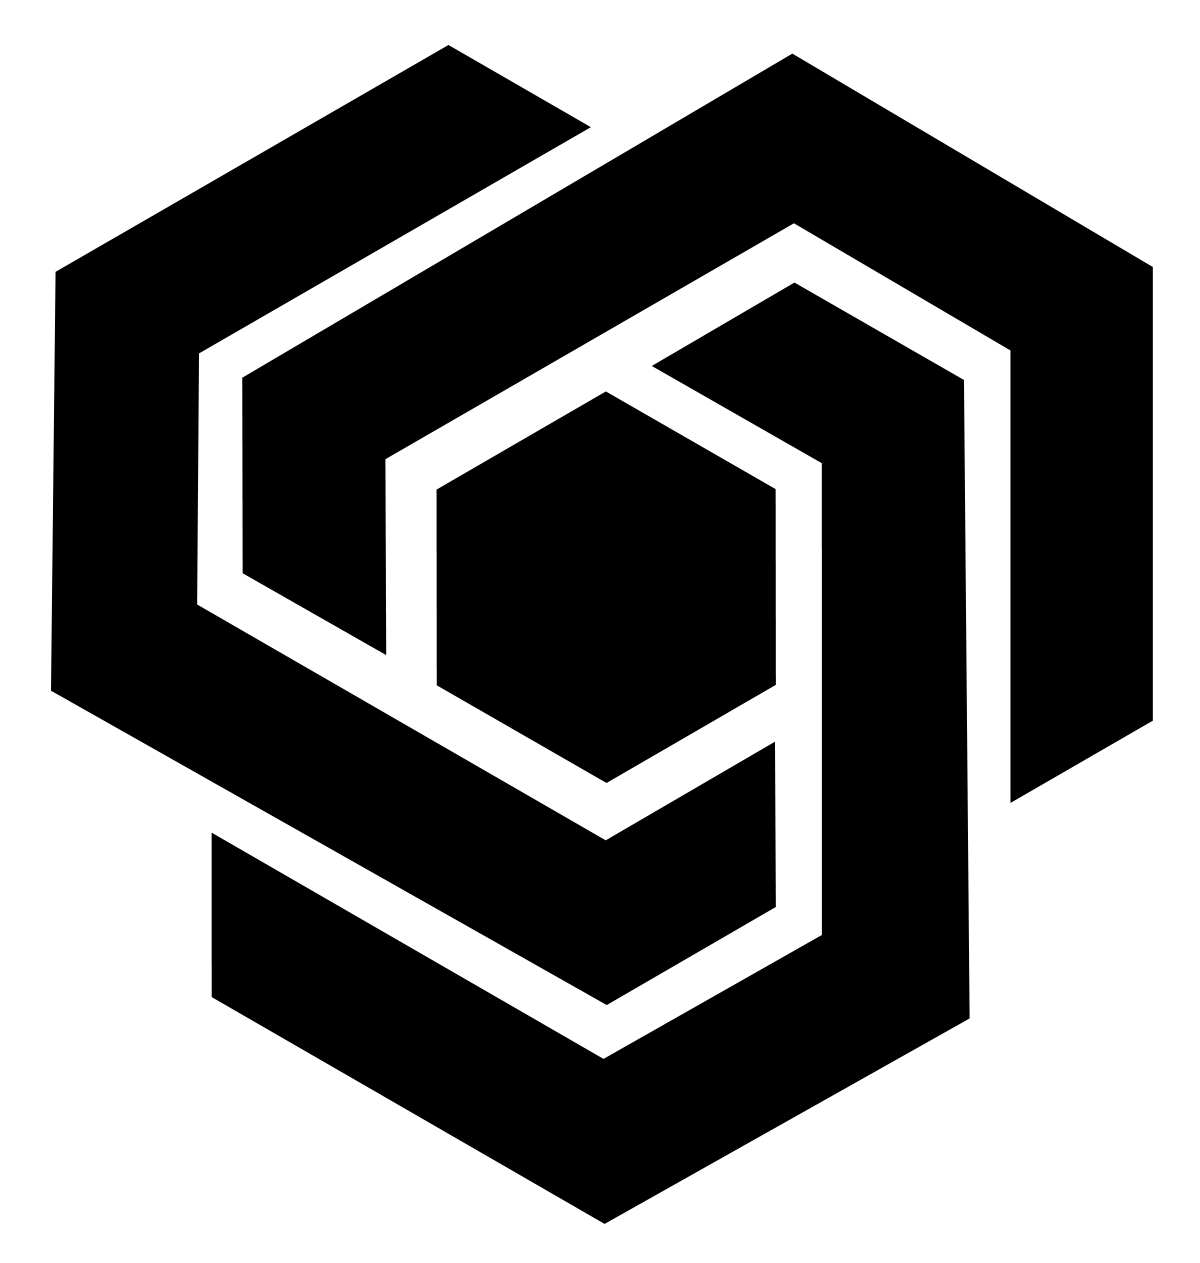
\includegraphics[width=0.2\textwidth]{Images/logo.png}} % Optional title page image, comment this line to remove it

\institute{Технически Университет София}

\date{25 Февруари 2022}

%------------------------------------------------
%\setlength{\parskip}{1.5em}
\linespread{1.25}



\begin{document}

%------------------------------------------------
	
\begin{frame}
	\begin{nohyphens}
	\maketitle % Automatically created using the information in the commands above
	\end{nohyphens}
\end{frame}

\section{Структура}
    
	
\begin{frame}
	\tableofcontents
\end{frame}

%----------------------------------------------------------------------------------------
%	 SECTION 1
%----------------------------------------------------------------------------------------

\section{Увод} 

\subsection{Цели и задачи - Софтуер}


\begin{frame}{Цели и задачи - Софтуер}
	\begin{itemize}
		\pause 
		\item Изграждане на среда за разработка на софтуер с основа \textit{Make} под \textit{Linux}

		\pause 
		\item Подбор на хардуерни и софтуерни решения за интеграция с разработената среда

		\pause 
		\item Създаване на софтуерни модули и драйвъри за работа с вътрешния и външен хардуер

		\pause 
		\item Подбор на изходни портове, пинове и нужна периферия

		\pause
		\item Инициализация и конфигурация на микроконтролера и периферията 

	\end{itemize}
\end{frame}

\subsection{Цели и задачи - Хардуер}


\begin{frame}{Цели и задачи - Хардуер}
	\begin{itemize}
		\pause 
		\item Оглед на съществуващия хардуер и подбор на компоненти за преизползване.

		\pause 
		\item Подбор нов на хардуер

		\pause 
		\item Разположение на хардуера и избор на конфигурация за системата 

		\pause 
		\item Подбор на изходни портове, пинове и нужна периферия

		\pause
		\item Свързване на компонентите и електроснабдяване

		\pause 
		\item Изграждане платформи за опитни постановки

		\pause 
		\item Сглобаване на системата

	\end{itemize}
\end{frame}

\subsection{Цели и задачи - Идентификация,\\ моделиране, наблюдение и управление}


\begin{frame}{Цели и задачи -  Идентификация,\\ моделиране, наблюдение и управление }
	\begin{itemize}
		\pause 
		\item Моделиране:

		\begin{itemize}
			\pause 
			\item Ротор с витло

			\pause 
			\item Платформа за управление на ъгъл на завъртане

			\pause 
			\item Платформа за безпилотен летателен апарат с четири ротора

		\end{itemize}
		\pause 
		\item Идентификация на параметри

		\pause 
		\item Компенсация на сензорни отмествания

		\pause
		\item Калибриране на сензорите

		\pause
		\item Синтез на наблюдател за оценка на ориентацията на платформата

		\pause 
		\item Синтез на управление
	\end{itemize}
\end{frame}


%------------------------------------------------

\section{Софтуерна част}

\subsection{Среда за разработка на софтуер с основа\\\textit{Make} под \textit{Linux}}


\begin{frame}{Описание и съставни части}
	\begin{columns}
		\column{0.7\textwidth}
		\begin{block}{ Състав на средата за работа под \textit{Linux}}
			\begin{itemize}
				\pause
				\item Система за насочено изграждане: \\ \textit{GNU Make}

				\pause
				\item \textbf{Kомпилатор:} \\ \textit{GCC ARM NON-EABI}

				\pause
				\item \textbf{Връзка с контролера:} \\ \textit{ST-LINK}

				\pause
				\item \textbf{Текстов редактор:} \\\textit{VIM + Ctags}

				\pause 
				\item \textbf{Дебъгер:} \\ \textit{GDB (GNU Project Debuger)} 

			\end{itemize}
		\end{block}
		\column{0.15\textwidth}
		\pause
			
\includegraphics[width=0.95\linewidth]{Images/make.png} \\[0.5em]
			
\includegraphics[width=0.95\linewidth]{Images/gcc.png}
		\column{0.15\textwidth}
			
\includegraphics[width=0.95\linewidth]{Images/st-link.png} \\[0.5em]
			
\includegraphics[width=0.95\linewidth]{Images/vim.png}\\[0.5em]
			
\includegraphics[width=0.95\linewidth]{Images/gdb.png}
	\end{columns}
\end{frame}

\begin{frame}{Команден итерфейс}

	\begin{block}{Подържани команди }
	\begin{description}
		\pause
		\item[make | make all] Цялостно изграждане чрез компилиране и свързване на всчики \emph{нужни} елементи.

		\pause
		\item[make clean] Изчистване на средата.

		\pause
		\item[make flash] Запис на изградения
		\footnote{В случай, че софтуерyt има нужда от (пре)изграждане, системата автоматично го (пре)изгражда.}
		софтуер в паметта на микроконтролера.

	\end{description}
	\end{block}
\end{frame}

\begin{frame}[t]
	\begin{block}{ }
	\begin{description}
		\pause
		\item[make debug] Отваряне на порт за дебъг, стартиране и свързване на дебъгера
		\footnote{Системата автоматино конфигурира дебъгера да използва дебъг символите в изградения софтуер.}

		\pause
		\item[make usart] Стартира интерактивен комуникационен интерфейс за връзка (IO) с контролера чрез USART.

		\pause
		\item[make usart\_read] Създава файл, съдържащ получените данни през USART порта.

	\end{description}
	\end{block}
\end{frame}


\begin{frame}{Подбрани хардуерни и софтуерни решения}
	\begin{columns}
		\column{0.7\textwidth}
		\begin{block}{ }
			\begin{itemize}
				\pause
				\item Логически анализатор и генератор на 
					\begin{itemize}
						\pause
						\item SQ50 - logic analyzer (IKALOGIC S.A.S)
						\pause
						\item ScanaStudio 16.04 (for Linux)
					\end{itemize}
				\pause
				\item UART / USB Конвертор + picocom
			\end{itemize}
		\end{block}
		\column{0.3\textwidth}
		\pause
		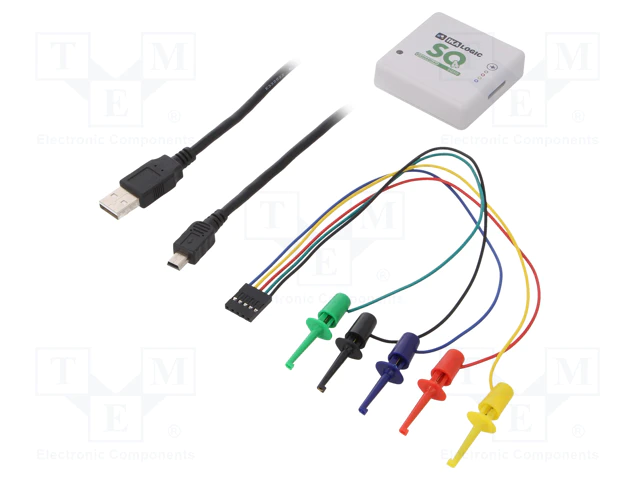
\includegraphics[width=0.8\linewidth]{Images/SQ50-logic-analyzer.png} \\[0.5em]
		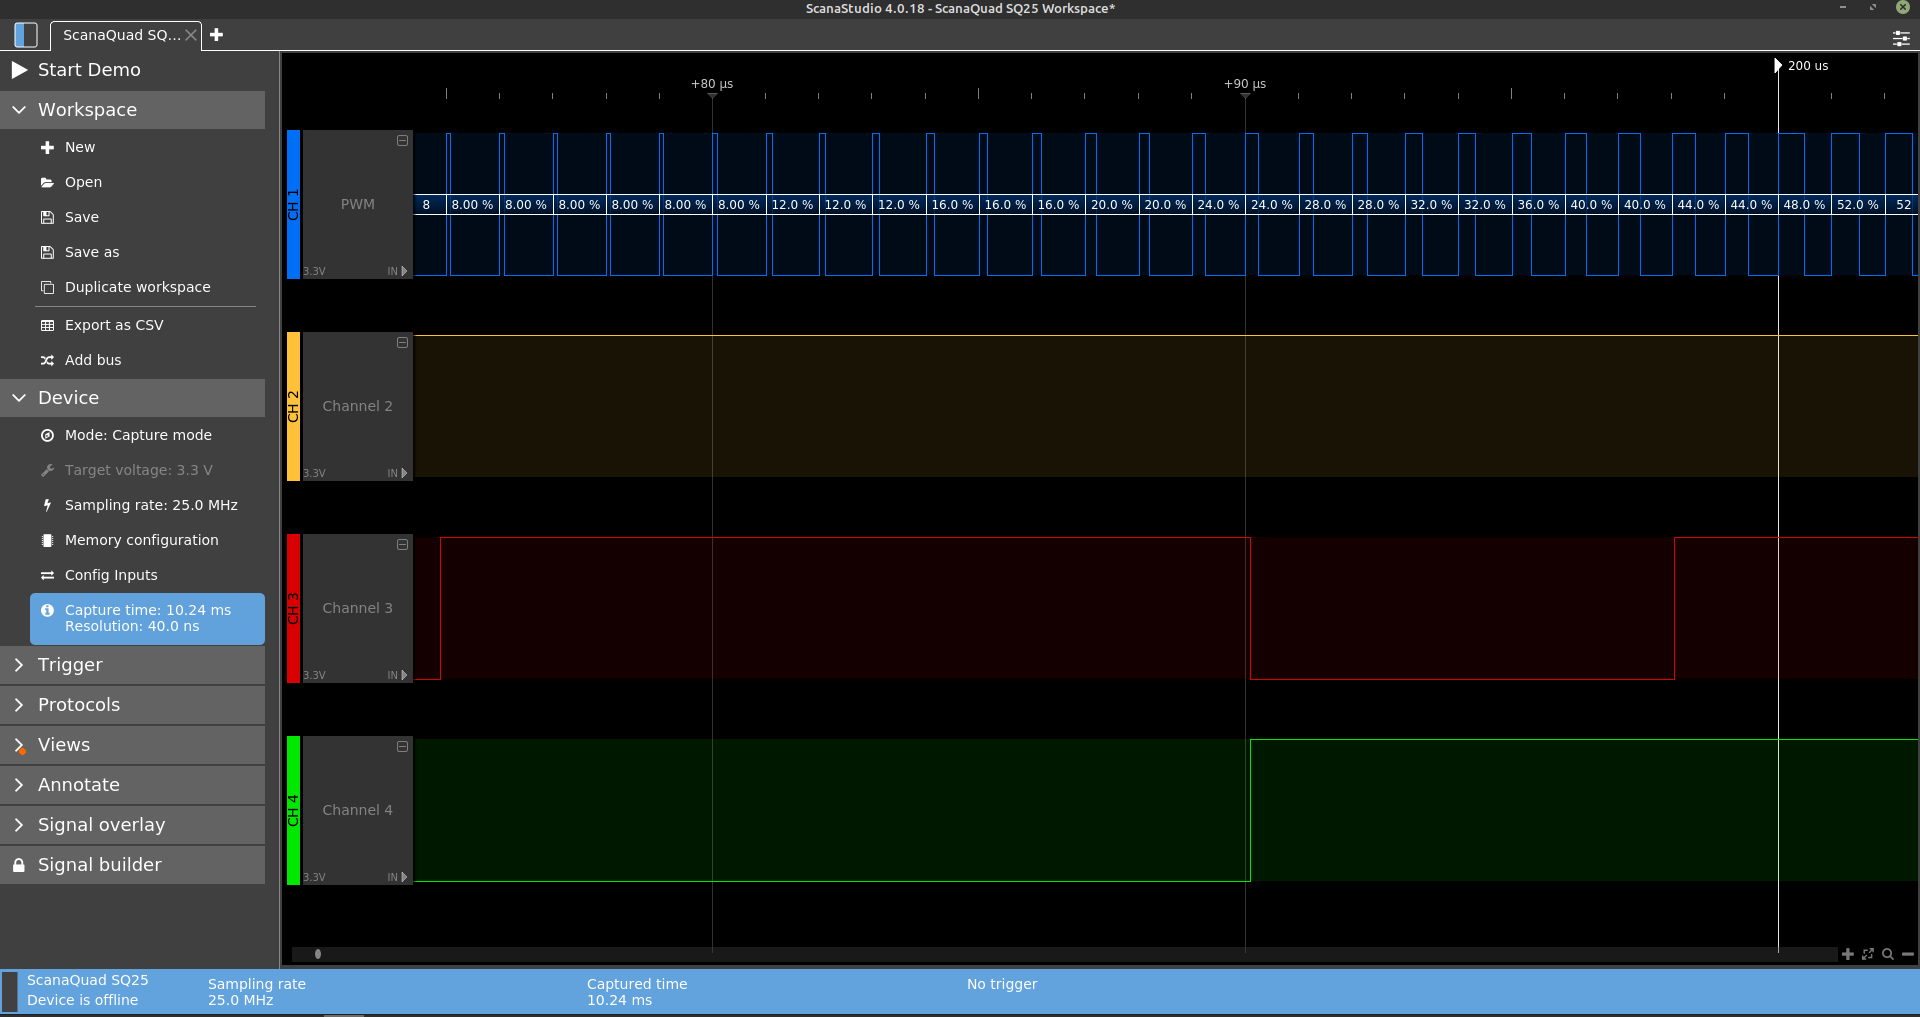
\includegraphics[width=0.8\linewidth]{Images/scana_studio_window.png}\\[0.5em]	
		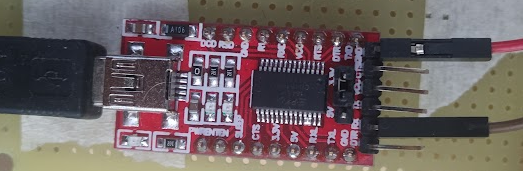
\includegraphics[width=0.9\linewidth]{Images/uart_usb.png} \\[0.5em]
	\end{columns}
\end{frame}

\subsection{Софтуерни модули за вътрешната и външна\\периферия}

\begin{frame}{Описание на модулите за вътрешна\\периферия}
	\pause
	Софтуерните модули са изградени на база описанието на регистирте за вътрешната периферия посочени в 
	Документът за Техническа справка на микроконтролери от семейство \textit{STM32F4xxx} \cite{stmcurefman}.\\[1.5em]

	\pause
	А основите за регистърните блокове на периферията в паметта е както е описано в дкоумента за съответният
	модел микроконтролер \cite{stmmcudatasheet}.

\end{frame}

\begin{frame}{Изградени модули за вътрешна периферия}
	\begin{block}{RCC (Reset and Clock Control)}
		Модул за управление на:
		\begin{itemize}
			\item Времеви баси (clock source: HSE, HSI, LSE)
			\item PLL честотен множител
			\item Делители на честота
			\item Часовниците на периферните шини
			\item Часовниците на периферията
		\end{itemize}
	\end{block}

\end{frame}

\begin{frame}

	\begin{block}{NVIC (Nested Vectored Interrupt Controller)}
		Модул за управление на:
		\begin{itemize}
			\item Конфигурацията на NVIC (контролера).
			\item Разрешаване и забрана на отделни прекъсвания.
			\item Маскиране на прекъсвания.
			\item Приоритет на прекъсванията
			\item Локацията на таблицата на прекъсванията.
		\end{itemize}
	\end{block}

\end{frame}

\begin{frame}

	\begin{block}{GPIO (General Purpose Input/Output)}
		Модул за управление на:
		 \begin{itemize}
			 \item Отделните GPIO портове.
			 \item Посока (изход/вход) за отделни пинове.
			 \item Pежим на работа на отделните пинове (Open-drain, Push-Pull, Analog, AF).
			 \item Вътрешни (Pull-up/Pull-down/Floating) конфигурации.
			 \item Източник за управление на състоянието на отделни пинове (Регистър / Алтернативна функция)
			 \item Работна честота на модула.
	 	\end{itemize}
	\end{block}

\end{frame}

\begin{frame}

	\begin{block}{TIM (Timers)}
		Модул за управление на прости таймери, таймери с общо предназначение и Специализирани таймери.
		Модула предоставя следните възможности:
		ААААААААААААААААААААААААААААААААААААААААААААААААААААААААААААААААААААААААААААААААААААААААААААААААААААААААААААААА
	\end{block}

\end{frame}

\begin{frame}[t]

	\begin{block}{I2C (Inter Integrated Circuit)}
		Модул за управление на конфигурацията на отделните I2C периферни модули.
		Предоставя ниво на абстракция позволяващa лесно четене и писане по регистрите на външни устройства, 
		като цялото управление на потока на комуникация е част от имплементираното прекъсване.
	\end{block}



\end{frame}

\section{Хардуерна част}


\section{Моделиране и Идентификация}

\subsection{Ротор с витло}

\begin{frame}{Моделиране на Ротор с витло}
	Опростен апроксимиран модел - нискочестотен филтър и коефициент на пропорционалност.
	\begin{figure}[htpb!]
		\centering
		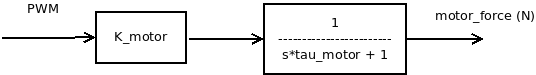
\includegraphics[width=0.7\textwidth]{Images/motor_model.png}
		\caption{Опростен модел на витло и мотор}
		\label{fig:motor_model}
	\end{figure}

	\begin{equation*}
		G_{motor}(s) = \frac{k_{motor}}{s \tau_{motor} + 1}
		\label{eqn:motor_model}
	\end{equation*}

\end{frame}

\begin{frame}{Снемане на характеристики на Ротор с витло}

\begin{figure}[htpb!]
    \centering
    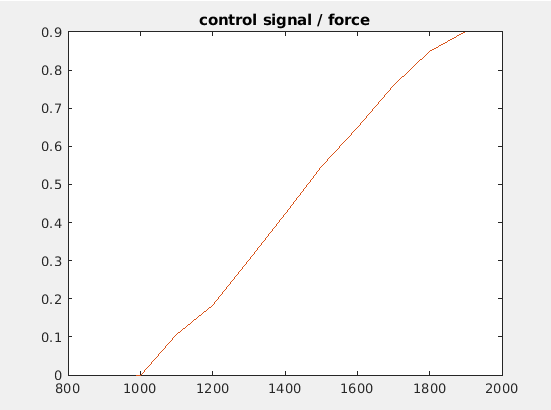
\includegraphics[width=0.6\textwidth]{Images/control_force.png}
\end{figure}


\(k_{motor} = 12.2e-3\) при сигнал \(1300\to1700\).

Опорната точка при тяга \(424g \approx 4.15N\)

\end{frame}

\subsection{Платформа за управление на ъгъл на\\ завъртане}

\begin{frame}{Моделиране на платформа за\\управление на ъгъл на завъртане}
	\begin{columns}
		\column{0.5\textwidth}

		Ако приемем:
		\begin{align*}
			F_2 &= F_0 + \delta f,F_1 &= F_0 - \delta f 
		\end{align*}
		И апроксимираме:
		\begin{align*}
			I &= \frac{l^2}{12}(M + 6m)
		\end{align*}\\[1em]

		\column{0.5\textwidth}
		
		\begin{figure}[htpb!]
			\centering
			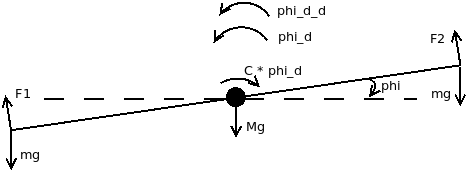
\includegraphics[width=0.9\textwidth]{Images/balance_force_diagram.png}
		\end{figure}

	\end{columns}

	Получаваме:
	\begin{equation*}
	G_{sys} = G_{motor}(s)G_{platform}(s) = 
	\frac{k_{motor} l}{s( s I + C)(s \tau_{motor} + 1)} 
	\end{equation*}

\end{frame}

\begin{frame}{Идентификация на параметри на \\ платформа за управление на ъгъл на \\завъртане}
	След снемане на преходен процес:
	\(I = 0.025, C = 0.018, \tau_{motor} = 0.08\)
			
	\begin{figure}[htpb!]
		\centering
		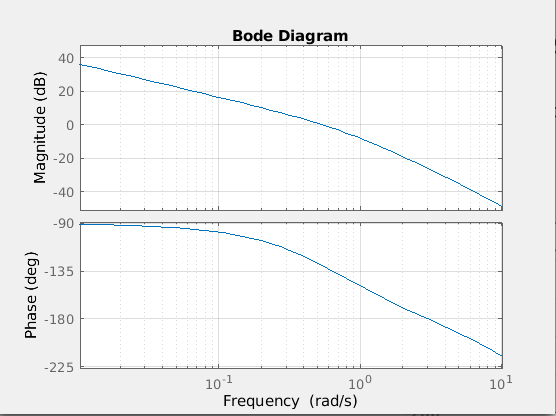
\includegraphics[width=0.5\textwidth]{Images/bode_balance.png}
	\end{figure}
\end{frame}


\subsection{Платформа за безпилотен летателен апарат с четири ротора}


\begin{frame}{}
AAAAAAAAAAAAAAAAAAAAAAAAAAAAAAAAAAAAAAAAAAAAAAAAAAAAAAAAAAAAAAAAAAA
\end{frame}

\section{Калибриране и компенсация}

\section{Синтез на наблюдател}

\section{Синтез на управление}




\begin{frame}[focus]
	Тази презентация е създадена с помощта на \textit{beamer} \LaTeX \textit{- Focus}
\end{frame}

\begin{frame}[focus]
	Специялни благодарности на \textit{Кристина Дойчева} за редакция и офрмление.
\end{frame}


%----------------------------------------------------------------------------------------
%	 CLOSING/SUPPLEMENTARY SLIDES
%----------------------------------------------------------------------------------------

\appendix

\begin{frame}{Литература}
	\nocite{*} % Display all references regardless of if they were cited
	\bibliography{example.bib}
	\bibliographystyle{plain}
\end{frame}

%------------------------------------------------

\begin{frame}{Backup Slide}
	This is a backup slide, useful to include additional materials to answer questions from the audience.
	\vfill
	The package \texttt{appendixnumberbeamer} is used to refrain from numbering appendix slides.
\end{frame}

%----------------------------------------------------------------------------------------

\end{document}
